\chapter{Results}
\label{sec:results}

In this chapter, we present five experiments run with two configurations of the MMO spacecraft. For the sake of brevity, we will refer to the case number as shown in table \ref{tab:MMOexperiments} when presenting analyses for these five experiments. Results will be presented in order such that the plasma conditions closest to those the MMO will actually experience when orbiting the MMO is presented as the last simulation where photoemission parameters are computed directly. Photoemission with a different electron temperature is also presented, since an assumption of constant photoelectron yield was assumed, the impact of a higher photoelectron temperature will be compared to the other experiments in which the average photoelectron temperature was computed using Planck's law. We have also chosen to group simulations with and without booms together to make comparison across the two configurations simpler.

Save for a computational charging analysis of the combined bepiColombo spacecraft under thrust (using the MTM, the Mercury Transfer Module) we were unable to find similar numerical experiments of the charging of the MMO spacecraft, we will therefore compare our results to theory through current balance analysis as presented in \ref{sec:theory}. As well as compare our results qualitatively to numerical charging experiments for different plasma parameters and different objects, such as in the paper by Deca et al. \parencite{Deca2013} used for our verification simulations.

From current balance, with photoemission included, we expect the variation of drift direction (comparing cases 2 and 3 to cases 7 and 8) to have minimal impact on the floating potential PINC will converge to, similarly we expect the sheath thickness and sheath plasma densities to be comparable for different drift directions. Across all five simulation types run, we expect the floating potential and sheath thickness to be larger in magnitude when the booms on the MMO are fully extended; since the booms are modeled as photoemissive, the greater surface area will lead to an overall higher electron current flowing from the spacecraft leading to a higher floating potential. 

The inclusion of the external magnetic field of Mercury could potentially impact the fraction of photoelectrons with a greater than average temperature being able to leave the surface of the spacecraft, if the particles' velocity vector does not align with the magnetic field the force exerted by the magnetic field could trap electrons more efficiently, leading to a lower floating potential.        



%FLOATING POTENTIAL SUMMARY
% \begin{table}[]
% \centering
% \begin{tabular}{cccccc}
% \hline
% & No photoelectron & Drift along Z & Drift along X & External Magnetic Field & Photoelectron temperature 3 eV\\\hline
% With booms & N/A & 105.419 & 105.400 & 105.400 & 78.154\\\hline
% Without booms & N/A & 100.710 & 100.696 & 100.699 & N/A\\\hline
% \end{tabular}
% \caption{Dummy text}
% \label{tab:FlotingPotSummary}
% \end{table}

\section{Charging without photoemission}
%FLOATING POTENTIAL CONVERGENCE
\begin{center}
    \begin{figure}[H]
      \begin{subfigure}[b]{0.75\textwidth}
      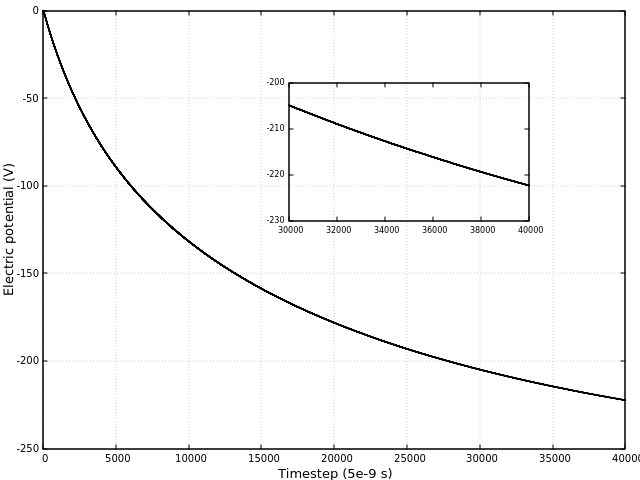
\includegraphics[width=\columnwidth]{figures/MMO/noPH/WB/C_noPH_WB.png}
      \caption{Booms}
      \label{fig:C_noPH_WB}
    \end{subfigure}
    \par\bigskip
    \begin{subfigure}[b]{0.75\textwidth}
      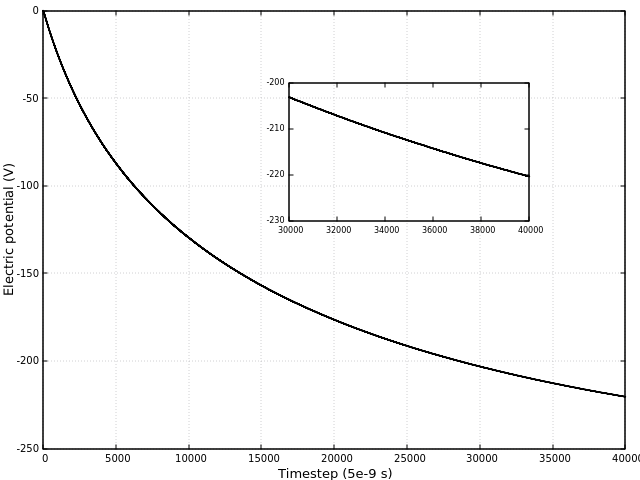
\includegraphics[width=\columnwidth]{figures/MMO/noPH/NB/C_noPH_NB.png}
      \caption{Without booms}
      \label{fig:C_noPH_NB}
    \end{subfigure}
  \label{fig:ConvnoPH}
  \caption{Timeseries plot of potential of the MMO with and without booms. The potential has been converted from PINC dimensionless units to Volts. The inset plots shows the potential of the two configurations for last 10,000 timesteps.}
  \end{figure}
\end{center}

The timeseries in fig \ref{fig:ConvnoPH} plots the potential of the MMO for each timestep simulated. From each inset plot, both for the MMO with booms and without, it is apparent from the slope that the system has not converged to a floating potential. Since the ambient plasma density around the MMO were approximately 100 times less dense than the value used in the verification simulation and no other current than ambient particle charging was present, a larger timestep was used in addition to a longer total simulation time. 

In order to compare our results with theory, we can estimate the floating potential the simulation would have converged to by fitting a function to our data and propagating the function forward in time until a steady state has been reached. Using Hill's function of the form 
\begin{equation*}
    \phi(t) = \phi_f \frac{t}{h + t},
\end{equation*}
where $\phi_f$ is the MMO floating potential without a photoemission current present, we estimate a floating potential of $\phi_f \approx 283 V$. A full analysis of the curve fitting and the Python script used to fit the curves is given in  \cref{sec:appendixC}.


%POTENTIAL THROUGH CENTER OF OBJECT
\begin{center}
    \begin{figure}[H]
      \begin{subfigure}[b]{0.61\textwidth}
      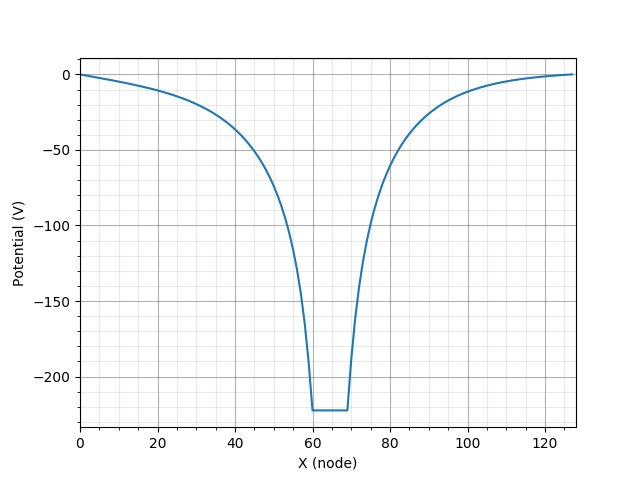
\includegraphics[width=\textwidth]{figures/MMO/noPH/WB/L_noPH_WB.png}
      \caption{Booms}
      \label{fig:L_noPH_WB}
    \end{subfigure}
    \begin{subfigure}[b]{0.61\textwidth}
      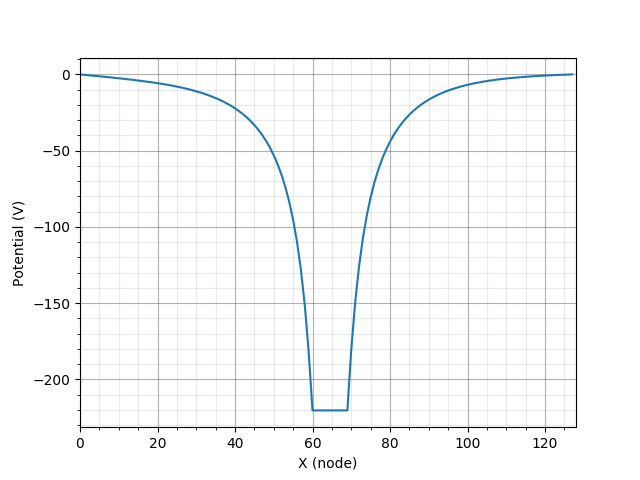
\includegraphics[width=\textwidth]{figures/MMO/noPH/NB/L_noPH_NB.png}
      \caption{Without booms}
      \label{fig:L_noPH_NB}
    \end{subfigure}
  \label{fig:Line_noPH}
  \caption{\ref{fig:L_noPH_NB} and \ref{fig:L_noPH_WB} show a potential profile along the X axis for the MMO without and with booms respectively. The line is plotted at $(x,y) = (13.95 m, 13.95 m)$, or node points $(x,y) = (62,62)$, and passes through the main octagonal body of the spacecraft. The X axis units are in number of nodes from the origin.}
  \end{figure}
\end{center}

Even without PINC converging to a floating potential, we can still make comparisons of the plasma sheath formed around the spacecraft by plotting the potential profile of the domain. Figure \ref{fig:Line_noPH}, shows the potential relative to the ambient plasma plotted on a center line passing through the spacecraft octohedral body. comparing figure \ref{fig:L_noPH_WB} with figure \ref{fig:L_noPH_NB}, we see a pre-sheath between node 0 and 20 (4.5 meters from the $X = 0$ wall) in the MMO configuration without booms. In figure \ref{fig:L_noPH_WB}, zero potential is only reached at the computational boundary, suggesting the sheath would physically extend beyond the defined computational domain.   





%AVERAGE POTENTIAL ISOLINES XY
\begin{center}
\begin{figure}[H]
  \begin{subfigure}[b]{0.61\textwidth}
    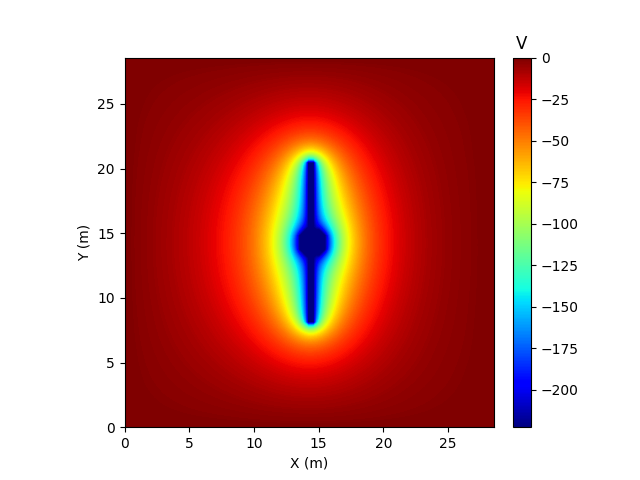
\includegraphics[width=\textwidth]{figures/MMO/noPH/WB/P_noPH_WB.png}
    \caption{Booms}
    \label{fig:P_noPH_WB}
  \end{subfigure}
  \hfill
  \begin{subfigure}[b]{0.61\textwidth}
    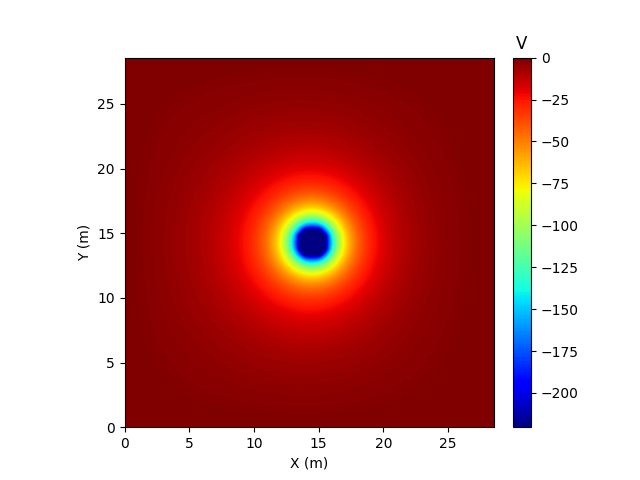
\includegraphics[width=\textwidth]{figures/MMO/noPH/NB/P_noPH_NB.png}
    \caption{Without booms}
    \label{fig:P_noPH_NB}
  \end{subfigure}
  \label{fig:Pot_noPH}
  \caption{\ref{fig:P_noPH_WB} and \ref{fig:P_noPH_WB} are 2D slice through $Z = 14.4 m$ showing the potential profile of the entire computational domain.}
\end{figure}
\end{center}

%PARTICLE DENSITIES (rho_i and rho_e)
%RHO_I
\begin{center}
    \begin{figure}[H]
      \begin{subfigure}[b]{0.61\textwidth}
      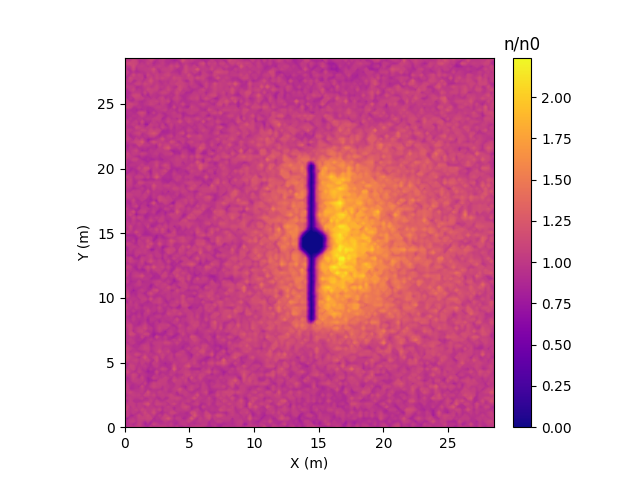
\includegraphics[width=\textwidth]{figures/MMO/noPH/WB/I_noPH_WB.png}
      \caption{Booms}
      \label{fig:I_noPH_WB}
    \end{subfigure}
    \begin{subfigure}[b]{0.61\textwidth}
      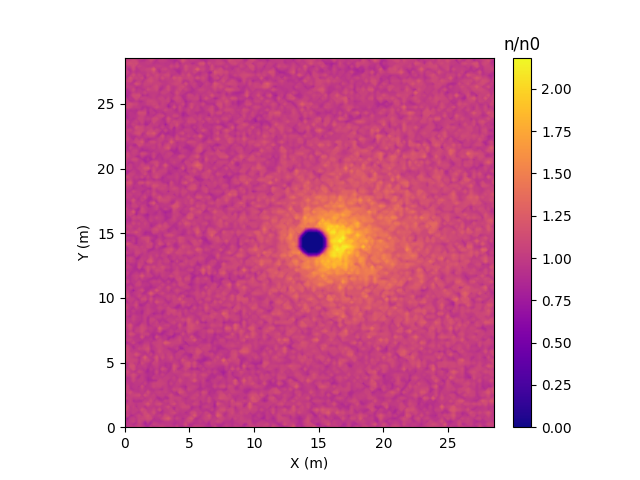
\includegraphics[width=\textwidth]{figures/MMO/noPH/NB/I_noPH_NB.png}
      \caption{Without booms}
      \label{fig:I_noPH_NB}
    \end{subfigure}
  \label{fig:Ions_noPH}
  \caption{Ion density profile plotted at $Z = 14.4 m$, the color gradient is normalized against the ion plasma density from table \ref{tab:PlasmaParamMMO}.}
  \end{figure}
\end{center}

%RHO_E
\begin{center}
    \begin{figure}[H]
      \begin{subfigure}[b]{0.61\textwidth}
      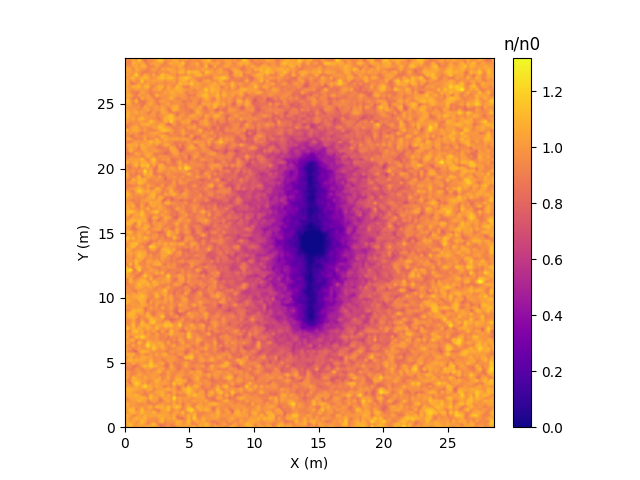
\includegraphics[width=\textwidth]{figures/MMO/noPH/WB/E_noPH_WB.png}
      \caption{Booms}
      \label{fig:E_noPH_WB}
    \end{subfigure}
    \begin{subfigure}[b]{0.61\textwidth}
      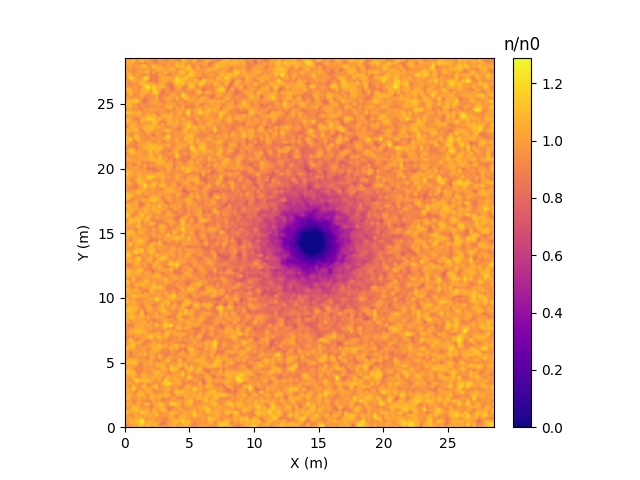
\includegraphics[width=\textwidth]{figures/MMO/noPH/NB/E_noPH_NB.png}
      \caption{Without booms}
      \label{fig:E_noPH_NB}
    \end{subfigure}
  \label{fig:Elec_noPH}
  \caption{Electron density profile plotted at $Z = 14.4 m$, the color gradient is normalized against the electron plasma density from table \ref{tab:PlasmaParamMMO}.}
  \end{figure}
\end{center}


\section{Charging with photoemission}

\subsection*{Drift parallel to X axis}

%FLOATING POTENTIAL CONVERGENCE
\begin{figure}[H]
  \centering
  \begin{subfigure}[b]{0.75\textwidth}
  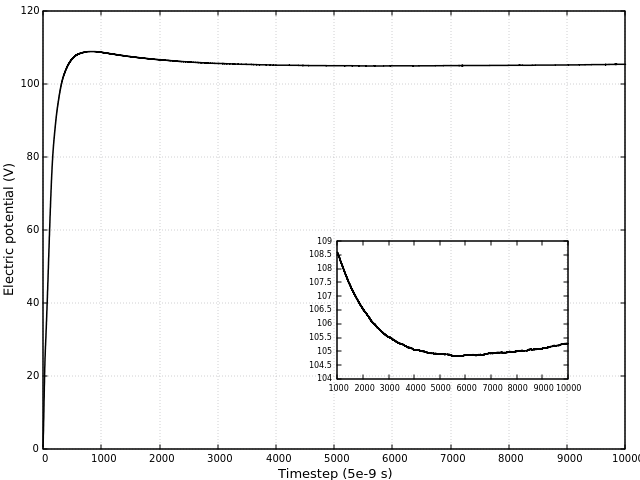
\includegraphics[width=\columnwidth]{figures/MMO/posX/WB/C_posX_WB.png}
  \caption{Booms}
  \label{fig:C_posX_WB}
\end{subfigure}
\hfill
\begin{subfigure}[b]{0.75\textwidth}
  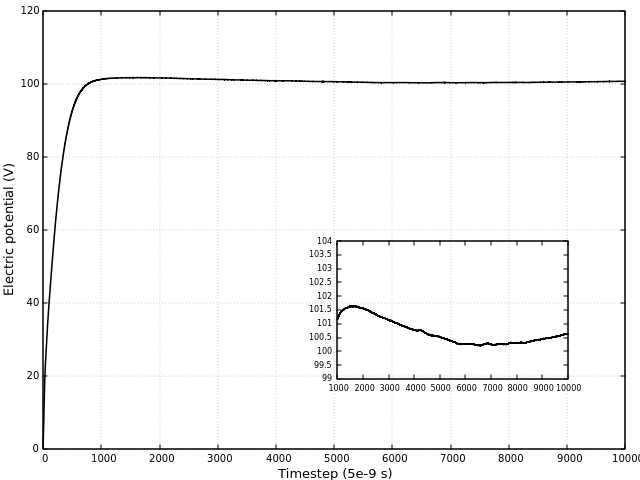
\includegraphics[width=\columnwidth]{figures/MMO/posX/NB/C_posX_NB.png}
  \caption{Without booms}
  \label{fig:C_posX_NB}
\end{subfigure}
\label{fig:Conv_posX}
\caption{Time series plot of the potential of the two MMO configurations for drift along X axis. The insets plots the same timeseries starting at 1000 timesteps, where the potential of the spacecraft has begun to oscillate about the floating potential.}
\end{figure}


%POTENTIAL THROUGH CENTER OF OBJECT

\begin{figure}[H]
  \begin{subfigure}[b]{0.6\textwidth}
  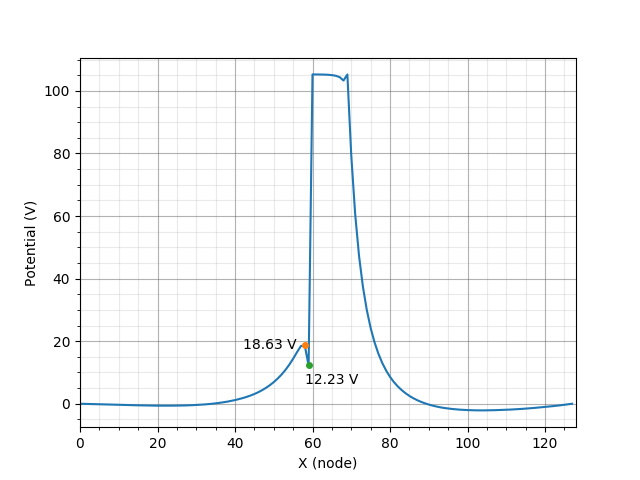
\includegraphics[width=\textwidth]{figures/MMO/posX/WB/L_posX_WB.png}
  \caption{Booms}
  \label{fig:L_posX_WB}
\end{subfigure}
\begin{subfigure}[b]{0.6\textwidth}
  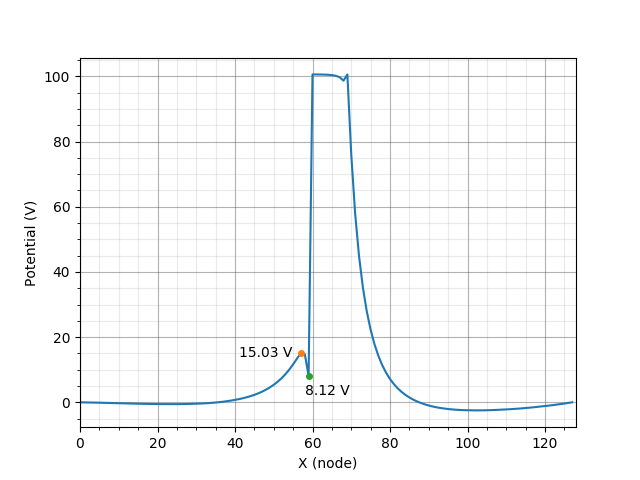
\includegraphics[width=\textwidth]{figures/MMO/posX/NB/L_posX_NB.png}
  \caption{Without booms}
  \label{fig:L_posX_NB}
\end{subfigure}
\label{fig:Line_posX}
\caption{Potential profile along the X axis for the two MMO configurations with drift along the X axis and photoemission included. The line is plotted at $(x,y) = (13.95 m, 13.95 m)$, or node points $(x,y) = (62,62)$, and passes through the main octagonal body of the spacecraft. The X axis units are in number of nodes from the origin. The two values in each plot show the height of the potential barrier formed.}
\end{figure}


%AVERAGE POTENTIAL ISOLINES XY

\begin{figure}[H]
  \begin{subfigure}[b]{0.6\textwidth}
    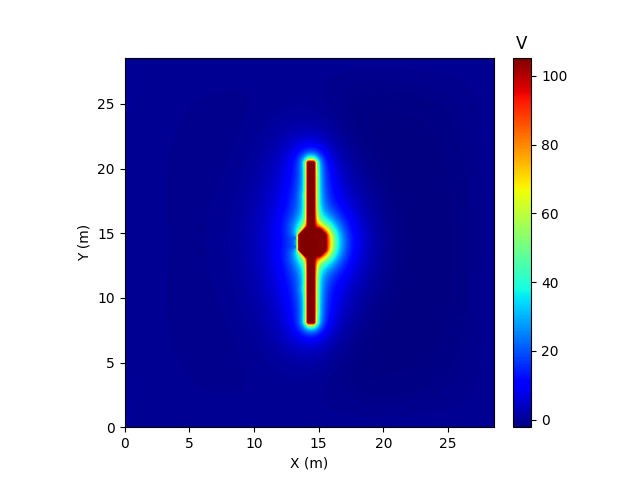
\includegraphics[width=\textwidth]{figures/MMO/posX/WB/P_posX_WB.png}
    \caption{Booms}
    \label{fig:P_posX_WB}
  \end{subfigure}
  \begin{subfigure}[b]{0.6\textwidth}
    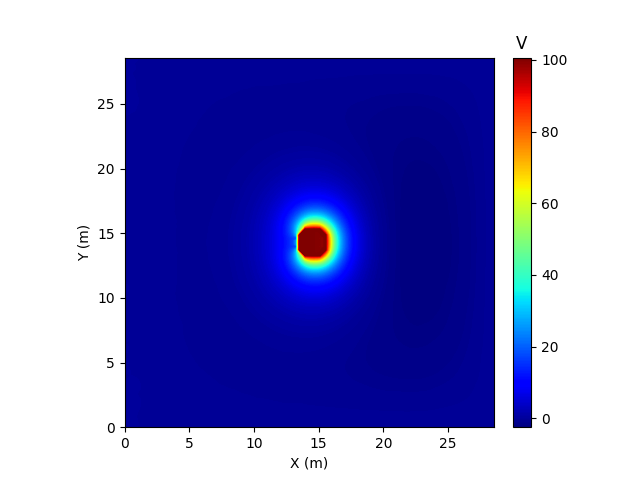
\includegraphics[width=\textwidth]{figures/MMO/posX/NB/P_posX_NB.png}
    \caption{Without booms}
    \label{fig:P_posX_NB}
  \end{subfigure}
  \label{fig:Pot_posX}
  \caption{2D slice through $Z = 14.4 m$ showing the time averaged potential profile of the entire computational domain with drift along X axis, and photoemission included. The potential is time averaged after a floating potential has been reached after 1,000 timesteps.}
\end{figure}



%PARTICLE DENSITIES (rho_i and rho_e)
%RHO_I

\begin{figure}[H]
  \begin{subfigure}[b]{0.6\textwidth}
  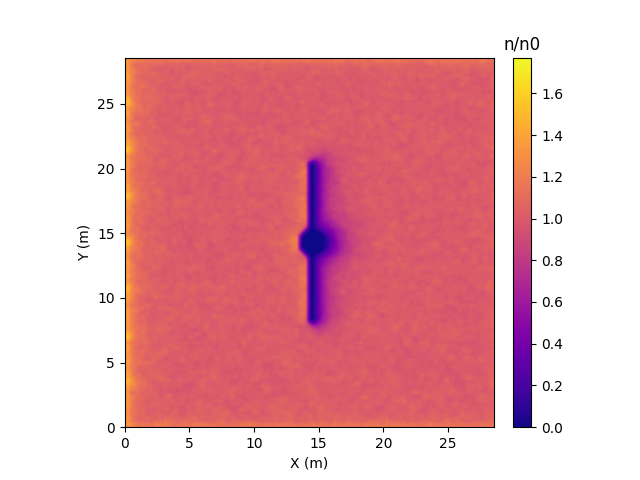
\includegraphics[width=\textwidth]{figures/MMO/posX/WB/I_posX_WB.png}
  \caption{Booms}
  \label{fig:I_posX_WB}
  \end{subfigure}
\begin{subfigure}[b]{0.6\textwidth}
  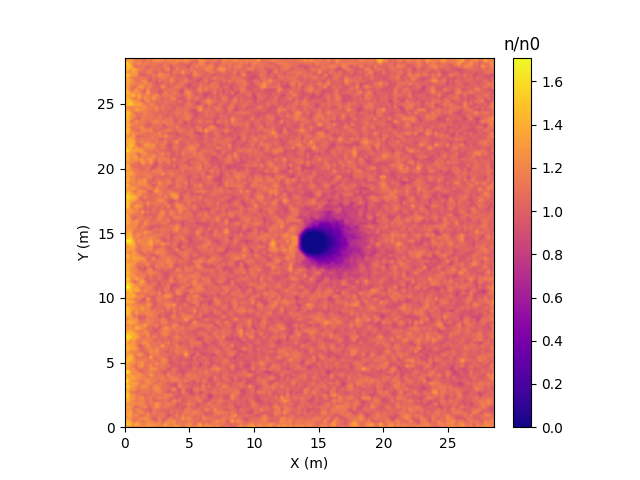
\includegraphics[width=\textwidth]{figures/MMO/posX/NB/I_posX_NB.png}
  \caption{Without booms}
  \label{fig:I_posX_NB}
\end{subfigure}
\label{fig:Ions_posX}
\caption{Ion density profile plotted at $Z = 14.4 m$, the color gradient is normalized against the ion plasma density from table \ref{tab:PlasmaParamMMO}. Plasma drift is along the X axis, and photoemission is included}
\end{figure}


%RHO_E

\begin{figure}[H]
  \begin{subfigure}[b]{0.6\textwidth}
  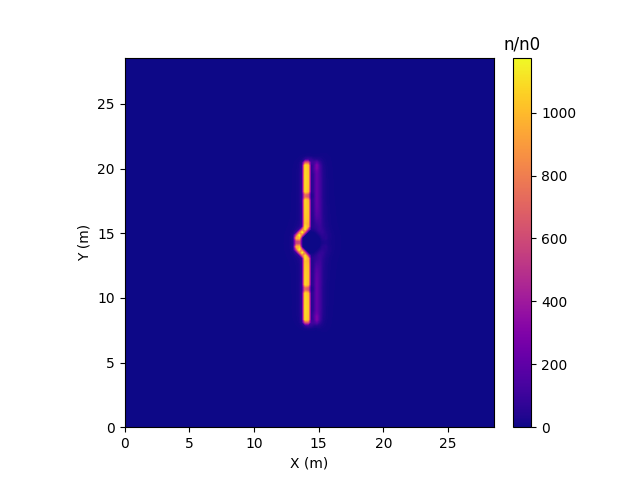
\includegraphics[width=\textwidth]{figures/MMO/posX/WB/E_posX_WB.png}
  \caption{Booms}
  \label{fig:E_posX_WB}
\end{subfigure}
\begin{subfigure}[b]{0.6\textwidth}
  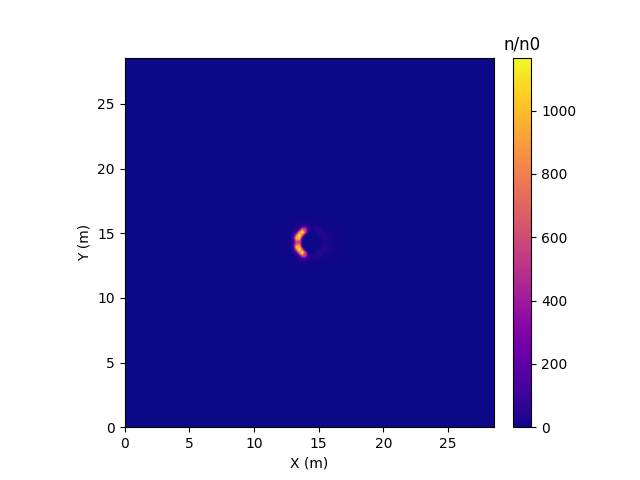
\includegraphics[width=\textwidth]{figures/MMO/posX/NB/E_posX_NB.png}
  \caption{Without booms}
  \label{fig:E_posX_NB}
\end{subfigure}
\label{fig:Elec_posX}
\caption{Electron density profile plotted at $Z = 14.4 m$, the color gradient is normalized against the electron plasma density from table \ref{tab:PlasmaParamMMO}. Drift is along the X axis, and photoemission is included, the sun is located in the negative X direction.}
\end{figure}




\subsection*{Drift parallel to Z axis}
%FLOATING POTENTIAL CONVERGENCE

\begin{figure}[H]
  \centering
  \begin{subfigure}[b]{0.75\textwidth}
  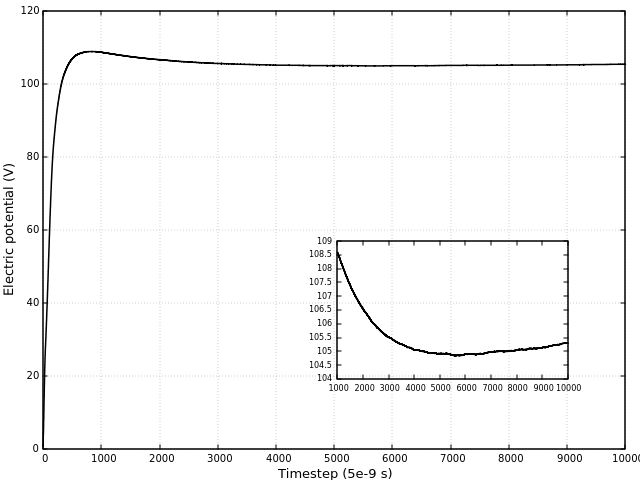
\includegraphics[width=\columnwidth]{figures/MMO/minZ/WB/C_minZ_WB.png}
  \caption{Booms}
  \label{fig:C_minZ_WB}
\end{subfigure}
\par\bigskip
\begin{subfigure}[b]{0.75\textwidth}
  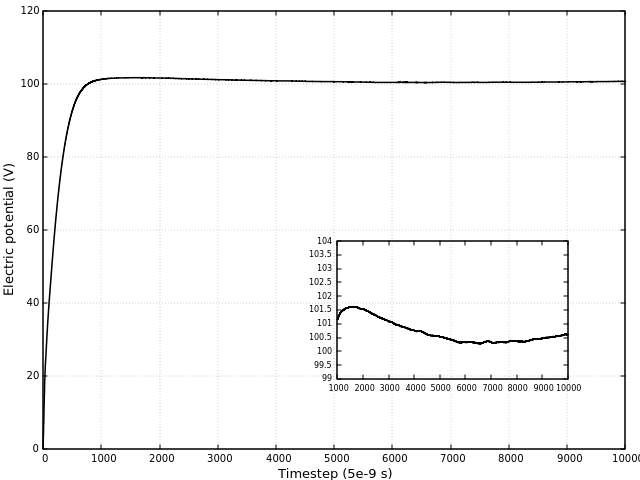
\includegraphics[width=\columnwidth]{figures/MMO/minZ/NB/C_minZ_NB.png}
  \caption{Without booms}
  \label{fig:C_minZ_NB}
\end{subfigure}
\label{fig:Conv_minZ}
\caption{Time series plot of the potential of the MMO with and without booms, where the drift is along the negative Z axis and photoemission is included. The inset plots the same timeseries after 1000 timesteps, where the potential of the spacecraft has begun to oscillate about the floating potential.}
\end{figure}


%POTENTIAL THROUGH CENTER OF OBJECT
\begin{figure}[H]
  \begin{subfigure}[b]{0.6\textwidth}
  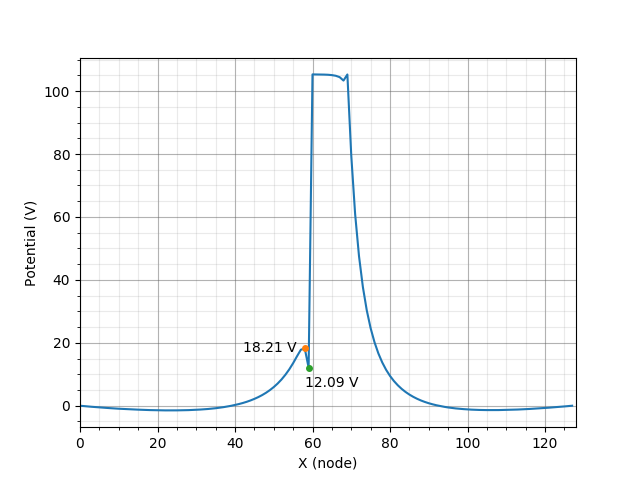
\includegraphics[width=\textwidth]{figures/MMO/minZ/WB/L_minZ_WB.png}
  \caption{Booms}
  \label{fig:L_minZ_WB}
\end{subfigure}
\begin{subfigure}[b]{0.6\textwidth}
  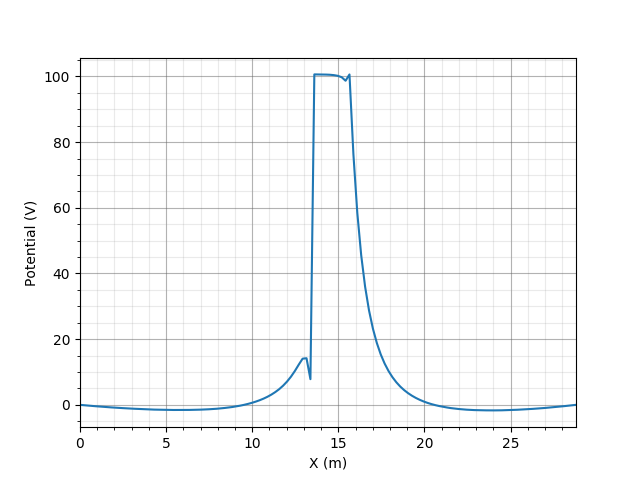
\includegraphics[width=\textwidth]{figures/MMO/minZ/NB/L_minZ_NB.png}
  \caption{Without booms}
  \label{fig:L_minZ_N}
\end{subfigure}
\label{fig:Line_minZ}
\caption{Potential profile along the X axis for the two MMO configurations with drift along the negative Z axis and photoemission included. The line is plotted at $(x,y) = (13.95 m, 13.95 m)$, or node points $(x,y) = (62,62)$, and passes through the main octagonal body of the spacecraft. The X axis units are in number of nodes from the origin. The two values in each plot show the height of the potential barrier formed.}
\end{figure}


%AVERAGE POTENTIAL ISOLINES XY
\begin{figure}[H]
  \begin{subfigure}[b]{0.6\textwidth}
    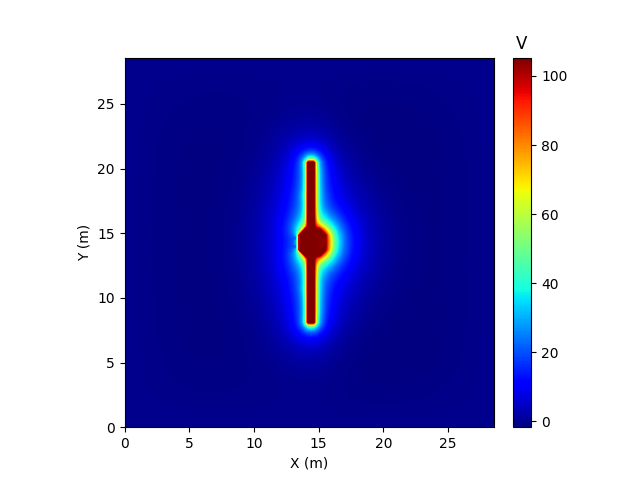
\includegraphics[width=\textwidth]{figures/MMO/minZ/WB/P_minZ_WB.png}
    \caption{Booms}
    \label{fig:P_minZ_WB}
  \end{subfigure}
  \hfill
  \begin{subfigure}[b]{0.6\textwidth}
    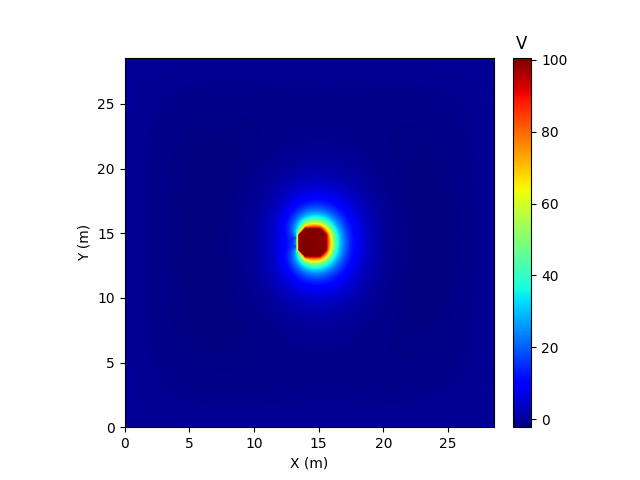
\includegraphics[width=\textwidth]{figures/MMO/minZ/NB/P_minZ_NB.png}
    \caption{Without booms}
    \label{fig:P_minZ_NB}
  \end{subfigure}
  \label{fig:Pot_minZ}
  \caption{2D slice through $Z = 14.4 m$ showing the time averaged potential profile of the entire computational domain with drift along the negative Z axis, and photoemission included. The potential is time averaged after a floating potential has been reached after 1,000 timesteps.}
\end{figure}

%PARTICLE DENSITIES (rho_i and rho_e)
%RHO_I
\begin{figure}[H]
  \begin{subfigure}[b]{0.6\textwidth}
  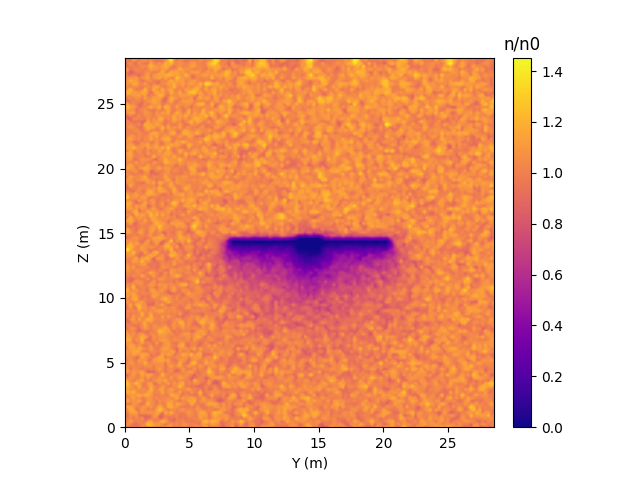
\includegraphics[width=\textwidth]{figures/MMO/minZ/WB/I_minZ_WB.png}
  \caption{Booms}
  \label{fig:I_minZ_WB}
\end{subfigure}
\begin{subfigure}[b]{0.6\textwidth}
  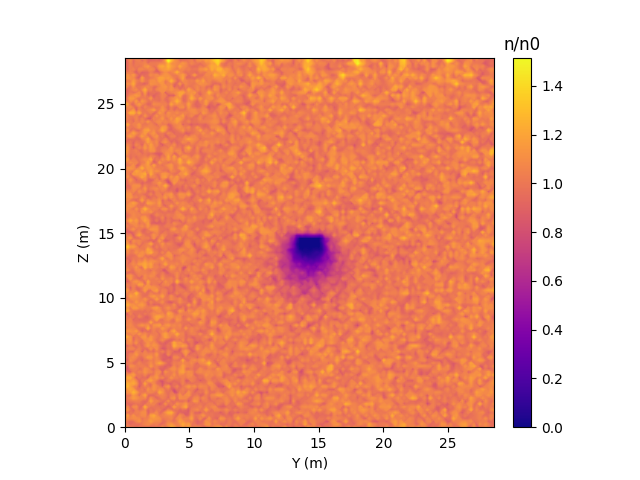
\includegraphics[width=\textwidth]{figures/MMO/minZ/NB/I_minZ_NB.png}
  \caption{Without booms}
  \label{fig:I_minZ_NB}
\end{subfigure}
\label{fig:Ion_minZ}
\caption{Ion density profile plotted at $Y = 14.4 m$, the color gradient is normalized against the ion plasma density from table \ref{tab:PlasmaParamMMO}. Drift is along the negative Z axis. and photoemission is included.}
\end{figure}

%RHO_E
\begin{figure}[H]
  \begin{subfigure}[b]{0.6\textwidth}
  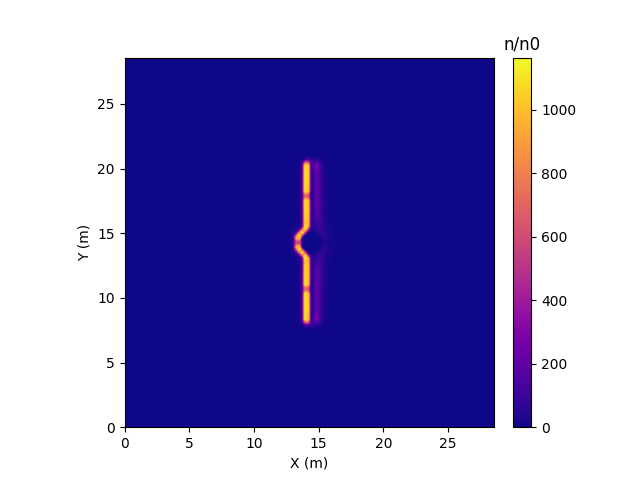
\includegraphics[width=\textwidth]{figures/MMO/minZ/WB/E_minZ_WB.png}
  \caption{Booms}
  \label{fig:E_minZ_WB}
\end{subfigure}
\begin{subfigure}[b]{0.6\textwidth}
  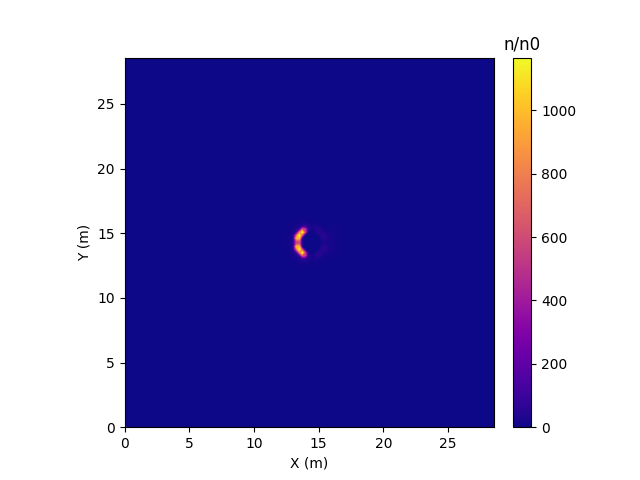
\includegraphics[width=\textwidth]{figures/MMO/minZ/NB/E_minZ_NB.png}
  \caption{Without booms}
  \label{fig:E_minZ_NB}
\end{subfigure}
\label{fig:Elec_minZ}
\caption{Electron density profile plotted at $Z = 14.4 m$, the color gradient is normalized against the electron plasma density from table \ref{tab:PlasmaParamMMO}. Drift is directed into the page, and photoemission is included. The sun is located in the negative X direction.}
\end{figure}


\section{Charging in an external magnetic field}

%FLOATING POTENTIAL CONVERGENCE
\begin{figure}[H]
  \begin{subfigure}[b]{0.75\textwidth}
  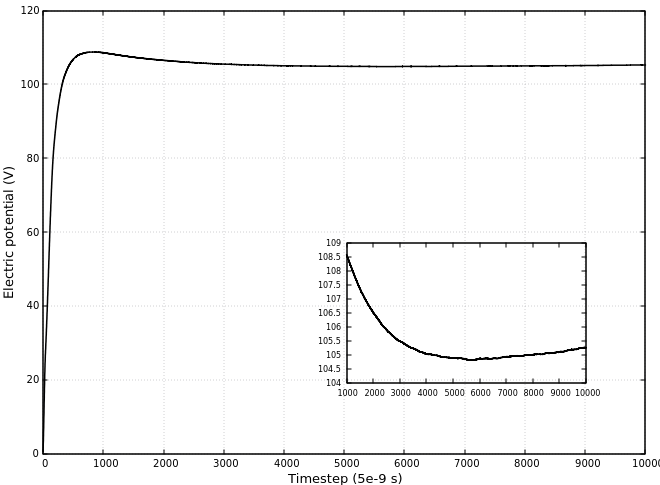
\includegraphics[width=\columnwidth]{figures/MMO/BField/WB/C_BField_WB.png}
  \caption{Booms}
  \label{fig:C_BField_WB}
\end{subfigure}
\par\bigskip
\begin{subfigure}[b]{0.75\textwidth}
  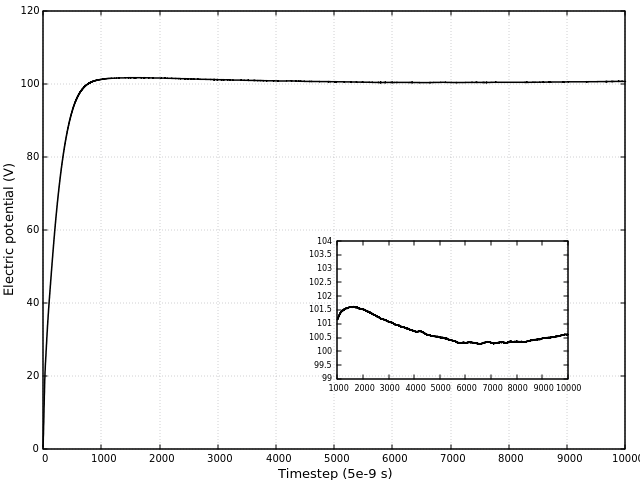
\includegraphics[width=\columnwidth]{figures/MMO/BField/NB/C_BField_NB.png}
  \caption{Without booms}
  \label{fig:C_BField_NB}
\end{subfigure}
\label{fig:Conv_BField}
\caption{Timeseries plot of the potential of the two configurations of the MMO, drift is along the negative Z axis, photoemission and an external magnetic field are included. The potential has been converted from PINC dimensionless units to Volts. The inset plots shows the potential of the two configurations for last 9,000 timesteps.}
\end{figure}


%POTENTIAL THROUGH CENTER OF OBJECT

\begin{figure}[H]
  \begin{subfigure}[b]{0.6\textwidth}
  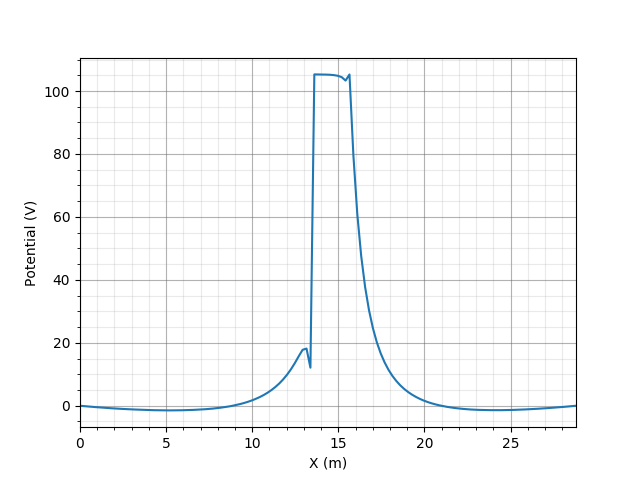
\includegraphics[width=\textwidth]{figures/MMO/BField/WB/L_BField_WB.png}
  \caption{Booms}
  \label{fig:L_BField_WB}
\end{subfigure}
\begin{subfigure}[b]{0.6\textwidth}
  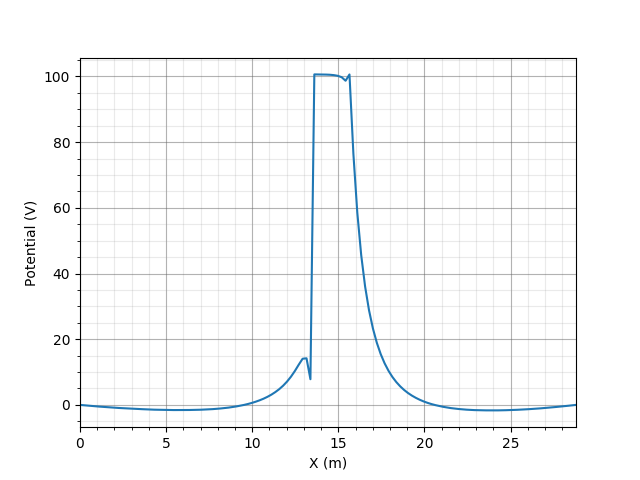
\includegraphics[width=\textwidth]{figures/MMO/BField/NB/L_BField_NB.png}
  \caption{Without booms}
  \label{fig:L_BField_NB}
\end{subfigure}
\label{fig:Line_BField}
\caption{Potential profile along the X axis for the two MMO configurations with drift along the negative Z axis, photoemission and an external magnetic field are included. The line is plotted at $(x,y) = (13.95 m, 13.95 m)$, or node points $(x,y) = (62,62)$, and passes through the main octagonal body of the spacecraft. The X axis units are in number of nodes from the origin. The two values in each plot show the height of the potential barrier formed.}
\end{figure}

%AVERAGE POTENTIAL ISOLINES XY
\begin{figure}[H]
  \begin{subfigure}[b]{0.6\textwidth}
    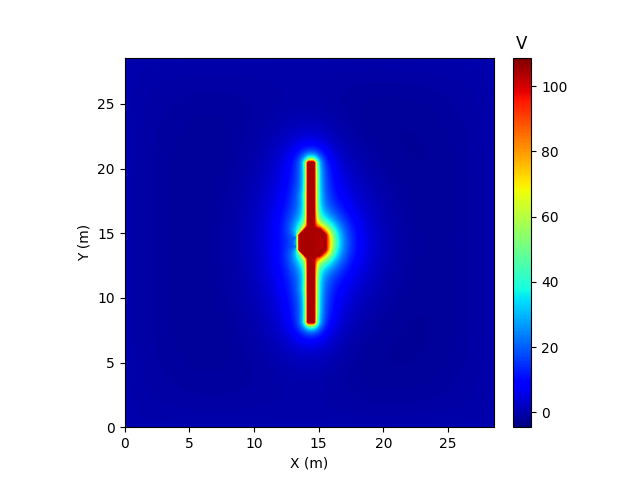
\includegraphics[width=\textwidth]{figures/MMO/BField/WB/P_BField_WB.png}
    \caption{Booms}
    \label{fig:P_BField_WB}
  \end{subfigure}
  \hfill
  \begin{subfigure}[b]{0.6\textwidth}
    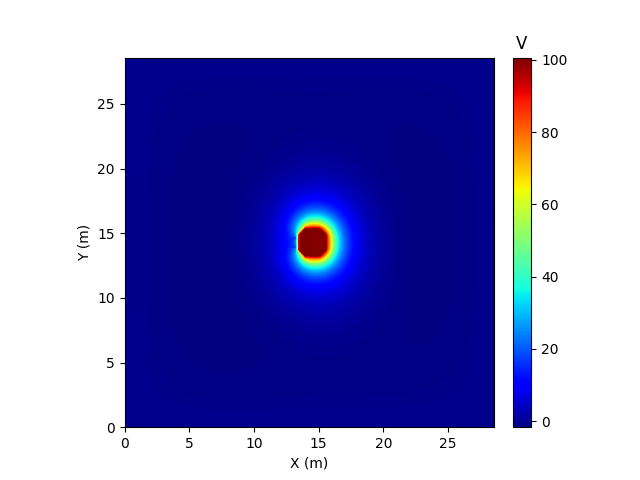
\includegraphics[width=\textwidth]{figures/MMO/BField/NB/P_BField_NB.png}
    \caption{Without booms}
    \label{fig:P_BField_NB}
  \end{subfigure}
  \label{fig:Pot_BField}
  \caption{2D slice through $Z = 14.4 m$ showing the time averaged potential profile of the entire computational domain with drift along the negative Z axis, photoemission and an external magnetic field are included. The potential is time averaged after a floating potential has been reached after 1,000 timesteps.}
\end{figure}

%PARTICLE DENSITIES (rho_i and rho_e)
%RHO_I
\begin{figure}[H]
  \begin{subfigure}[b]{0.6\textwidth}
  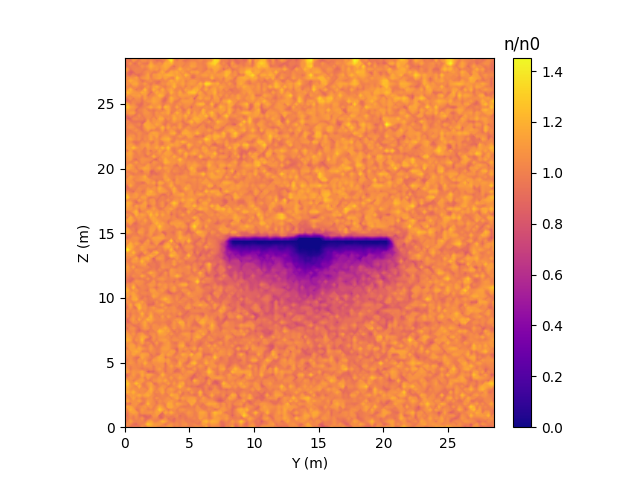
\includegraphics[width=\textwidth]{figures/MMO/BField/WB/I_BField_WB.png}
  \caption{Booms}
  \label{fig:I_BField_WB}
\end{subfigure}
\begin{subfigure}[b]{0.6\textwidth}
  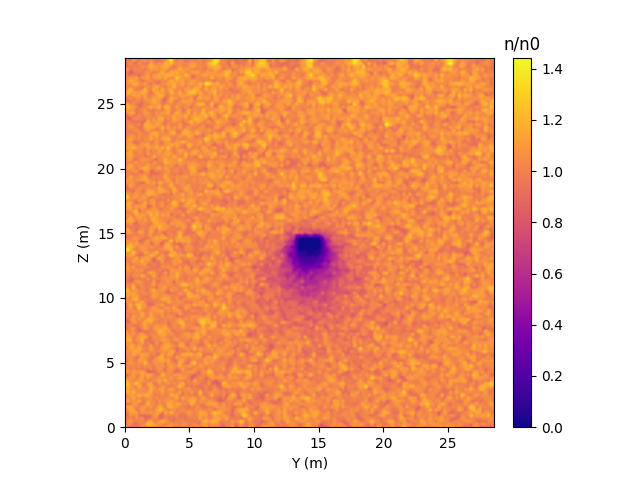
\includegraphics[width=\textwidth]{figures/MMO/BField/NB/I_BField_NB.png}
  \caption{Without booms}
  \label{fig:I_BField_NB}
\end{subfigure}
\label{fig:Ions_BField}
\caption{Ion density profile plotted at $Z = 14.4 m$, the color gradient is normalized against the ion plasma density from table \ref{tab:PlasmaParamMMO}. Drift is along the negative Z axis, photoemission and an external magnetic field are included.}
\end{figure}

%RHO_E
\begin{figure}[H]
  \begin{subfigure}[b]{0.6\textwidth}
  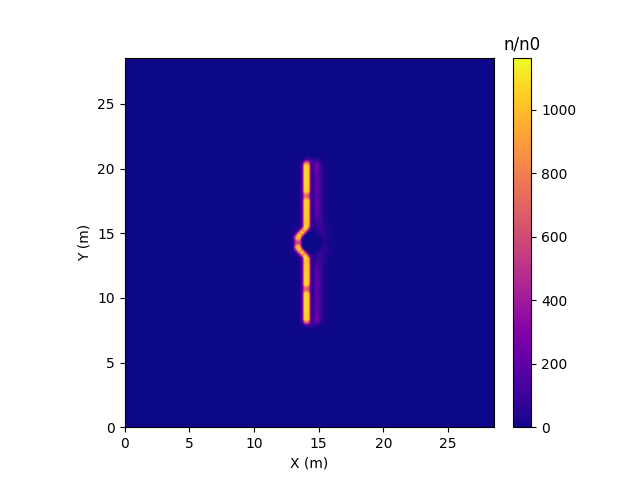
\includegraphics[width=\textwidth]{figures/MMO/BField/WB/E_BField_WB.png}
  \caption{Booms}
  \label{fig:E_BField_WB}
\end{subfigure}
\begin{subfigure}[b]{0.6\textwidth}
  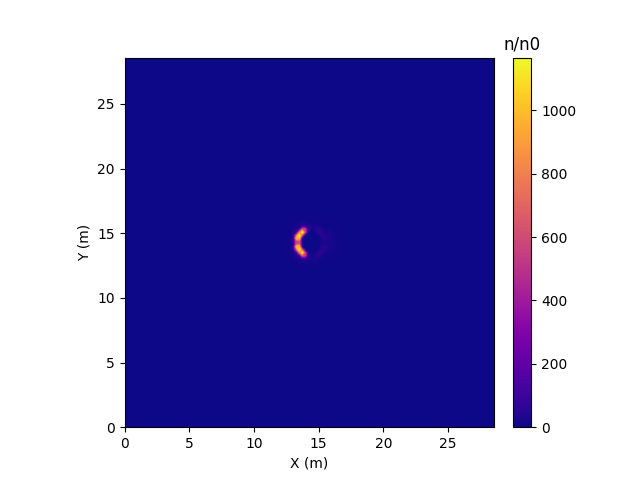
\includegraphics[width=\textwidth]{figures/MMO/BField/NB/E_BField_NB.png}
  \caption{Without booms}
  \label{fig:E_BField_NB}
\end{subfigure}
\label{fig:Elec_BField}
\caption{Electron density profile plotted at $Z = 14.4 m$, the color gradient is normalized against the electron plasma density from table \ref{tab:PlasmaParamMMO}.Drift is along the negative Z axis, photoemission and an external magnetic field are included. The direction of the sun is along the negative X axis.}
\end{figure}

\section{Charging at different photoelectron temperatures}

%FLOATING POTENTIAL CONVERGENCE
\begin{figure}[H]
  \centering
  \begin{subfigure}[b]{0.75\textwidth}
  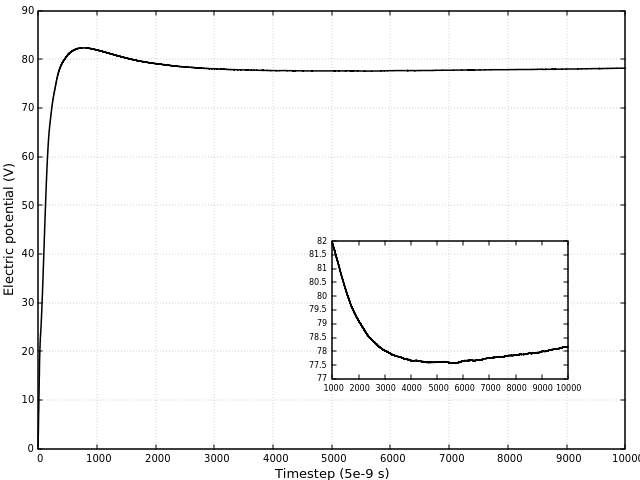
\includegraphics[width=\columnwidth]{figures/MMO/PHTemp/WB/C_PHTemp_WB.png}
  \caption{Booms}
  \label{fig:C_PHTemp_WB}
\end{subfigure}
\par\bigskip
\begin{subfigure}[b]{0.75\textwidth}
  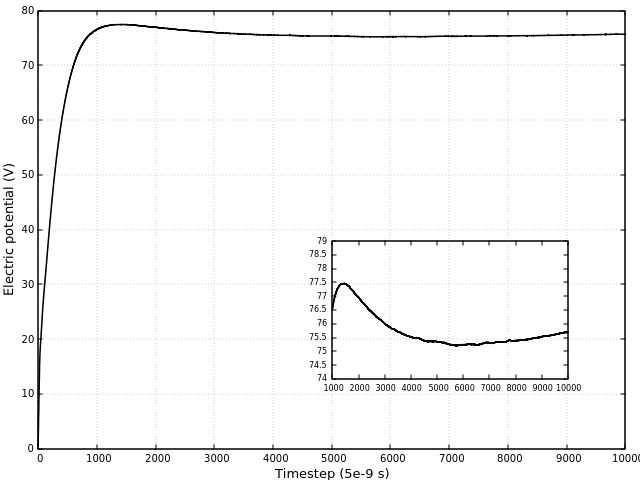
\includegraphics[width=\columnwidth]{figures/MMO/PHTemp/NB/C_PHTemp_NB.png}
  \caption{Without booms}
  \label{fig:C_PHTemp_NB}
\end{subfigure}
\label{fig:Conv_PHTemp}
\caption{Timeseries plot of the potential of the two configurations of the MMO, drift is along the negative Z axis and the photoelectron temperature has been set to $3 \; eV$. The potential has been converted from PINC dimensionless units to Volts. The inset plots the same timeseries after 1000 timesteps, where the potential of the spacecraft has begun to oscillate about the floating potential.}
\end{figure}

%POTENTIAL THROUGH CENTER OF OBJECT
\begin{figure}[H]
  \begin{subfigure}[b]{0.6\textwidth}
  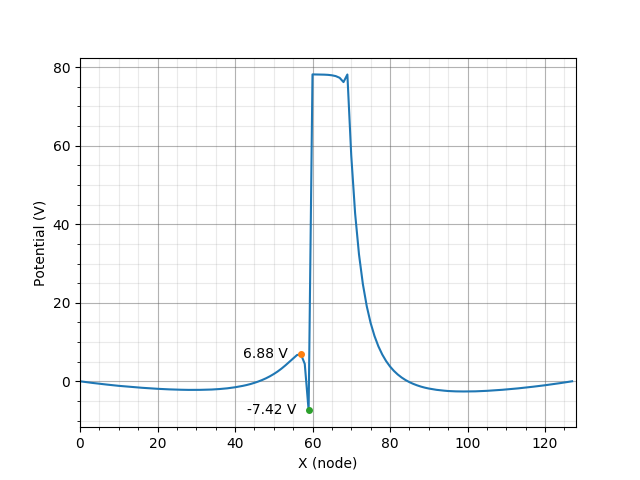
\includegraphics[width=\textwidth]{figures/MMO/PHTemp/WB/L_PHTemp_WB.png}
  \caption{Booms}
  \label{fig:L_PHTemp_WB}
\end{subfigure}
\begin{subfigure}[b]{0.6\textwidth}
  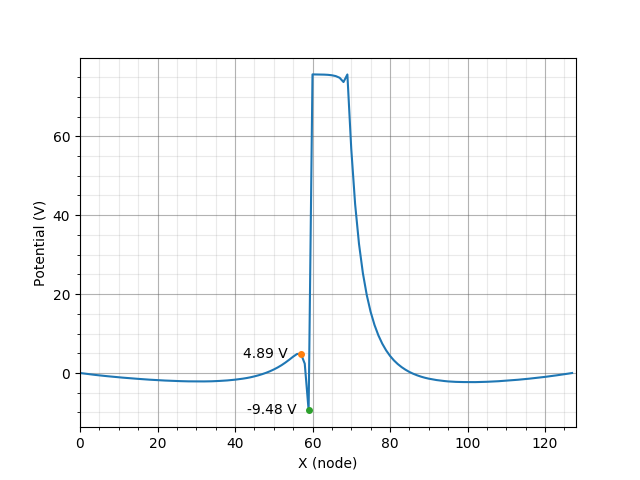
\includegraphics[width=\textwidth]{figures/MMO/PHTemp/NB/L_PHTemp_NB.png}
  \caption{Without booms}
  \label{fig:L_PHTemp_NB}
\end{subfigure}
\label{fig:Line_PHTemp}
\caption{Potential profile along the X axis for the two MMO configurations with drift along the negative Z axis, photoemission is included with a photoelectron temperature of $3 \; eV$. The line is plotted at $(x,y) = (13.95 m, 13.95 m)$, or node points $(x,y) = (62,62)$, and passes through the main octagonal body of the spacecraft. The X axis units are in number of nodes from the origin. The two values in each plot show the height of the potential barrier formed.}
\end{figure}

%AVERAGE POTENTIAL ISOLINES XY
\begin{figure}[H]
  \begin{subfigure}[b]{0.6\textwidth}
    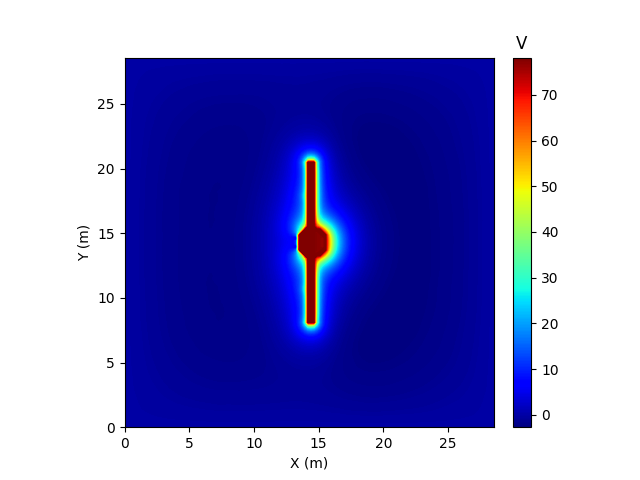
\includegraphics[width=\textwidth]{figures/MMO/PHTemp/WB/P_PHTemp_WB.png}
    \caption{Booms}
    \label{fig:P_PHTemp_WB}
  \end{subfigure}
  \hfill
  \begin{subfigure}[b]{0.6\textwidth}
    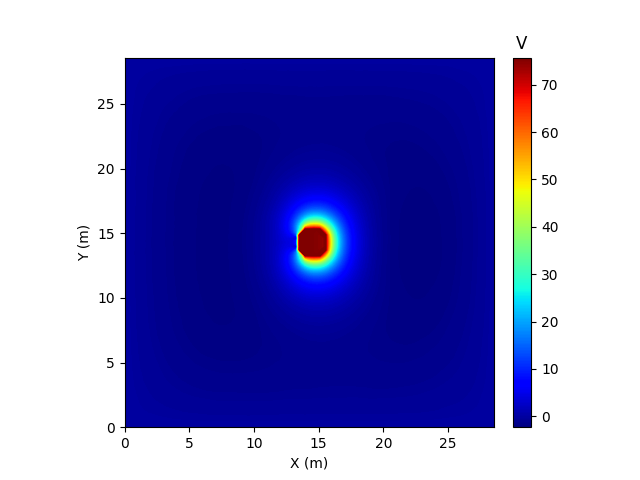
\includegraphics[width=\textwidth]{figures/MMO/PHTemp/NB/P_PHTemp_NB.png}
    \caption{Without booms}
    \label{fig:P_PHTemp_NB}
  \end{subfigure}
  \label{fig:Pot_PHTemp}
  \caption{2D cut through $Z = 14.4 m$ showing the time averaged potential profile of the entire computational domain with drift along the negative Z axis, photoemission is included with a photoelectron temperature of $3 \; eV$. The potential is time averaged after a floating potential has been reached after 1,000 timesteps.}
\end{figure}

%PARTICLE DENSITIES (rho_i and rho_e)
%RHO_I
\begin{figure}[H]
  \begin{subfigure}[b]{0.6\textwidth}
  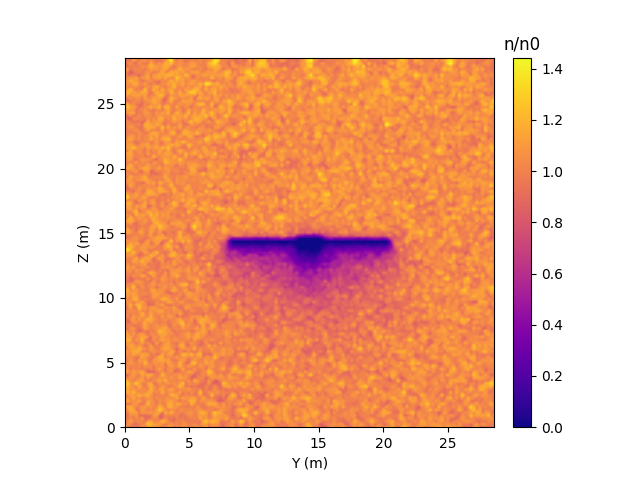
\includegraphics[width=\textwidth]{figures/MMO/PHTemp/WB/I_PHTemp_WB.png}
  \caption{Booms}
  \label{fig:I_PHTemp_WB}
\end{subfigure}
\begin{subfigure}[b]{0.6\textwidth}
  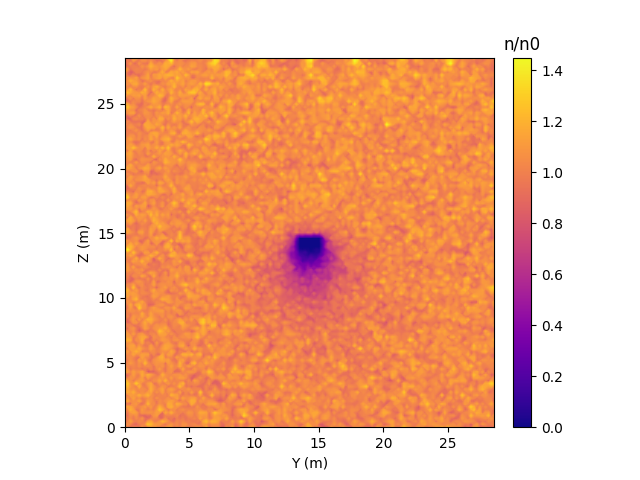
\includegraphics[width=\textwidth]{figures/MMO/PHTemp/NB/I_PHTemp_NB.png}
  \caption{Without booms}
  \label{fig:I_PHTemp_NB}
\end{subfigure}
\label{fig:Ions_PHTemp}
\caption{Ion density profile plotted at $Z = 14.4 m$, the color gradient is normalized against the ion plasma density from table \ref{tab:PlasmaParamMMO}. Drift is along the negative Z axis, and photoemission is included with a photoelectron temperature of $3 \; eV$.}
\end{figure}

%RHO_E
\begin{figure}[H]
  \begin{subfigure}[b]{0.6\textwidth}
  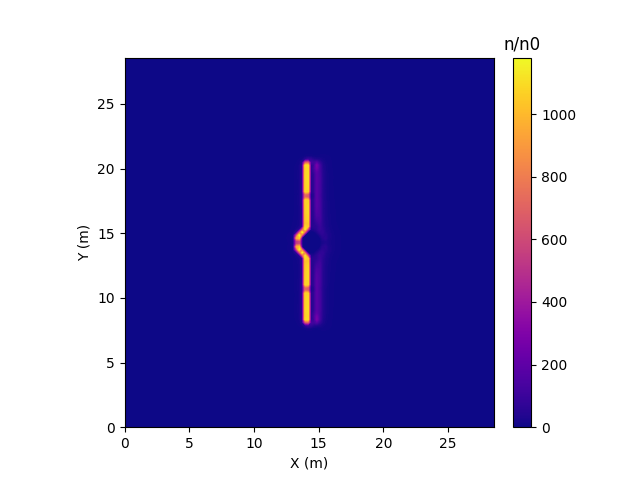
\includegraphics[width=\textwidth]{figures/MMO/PHTemp/WB/E_PHTemp_WB.png}
  \caption{Booms}
  \label{fig:E_PHTemp_WB}
\end{subfigure}
\begin{subfigure}[b]{0.6\textwidth}
  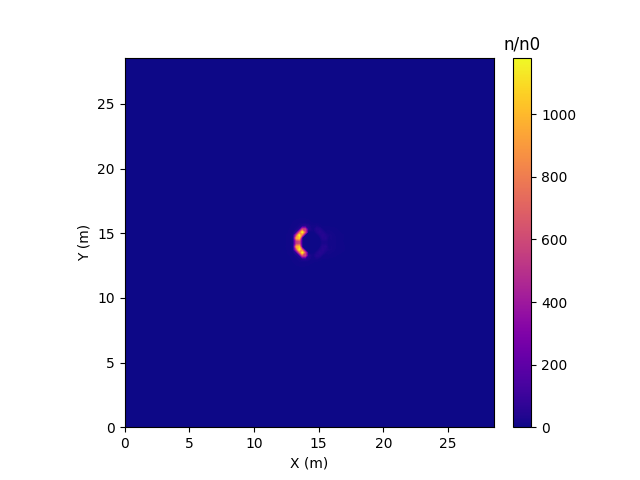
\includegraphics[width=\textwidth]{figures/MMO/PHTemp/NB/E_PHTemp_NB.png}
  \caption{Without booms}
  \label{fig:E_PHTemp_NB}
\end{subfigure}
\label{fig:Elec_PHTemp}
\caption{Electron density profile plotted at $Z = 14.4 m$, the color gradient is normalized against the electron plasma density from table \ref{tab:PlasmaParamMMO}. Drift is along the negative Z axis, and photoemission is included with a photoelectron temperature of $3 \; eV$.}
\end{figure}